\subsection{Execution Semantics}
In this subsection, we describe the execution semantics of \bcool, \ie how a \bcool specification is used to obtain a coordination model. We illustrate the different steps in the generation by using the specification presented in Listing~\ref{lst:bcoolrunningexample} to coordinate the models of the coffee machine (see Figure~\ref{fig:semantics})

Let $Ev$ be the (finite) set of event type names (representing the \dse). Considering a language $L$, A behavioral interface $i_L$ is a subset of event type names, $i_L \subset Ev$. A \bcool specification imports $N$ disjoint language interfaces and a set of operators $\mathcal{O}p$, with $N\geq 2$. Each operator from $\mathcal{O}p$ has a set of formal parameters $\mathcal{P}$, where each parameter is defined by a name and its type (\ie an event type). Each operator also has a correspondence matching condition (denoted $CMC$) and a correspondence rule (denoted $CR$). A \bcool specification is applied to a set of input models denoted $\mathcal{M_I}$, with $|\mathcal{M_I}| = N$.

From an operational point of view, the first step consists in producing the model behavioral interface of each input model. It results in a set of model interfaces denoted $\mathcal{I_{M_I}}$, of size $N$. An interface is a set of events, each of which is typed by an event type. For example, for the models of the coffee machine, step 1 in Figure~\ref{fig:semantics} shows the \mse of each model behavioral interface.  

Each operator $op$ in $\mathcal{O}p$ is processed individually and several times with different actual parameters, which depend on the model interfaces in $\mathcal{I_{M_I}}$. The set of actual parameters to be used is obtained by a \emph{restricted} Cartesian product of all the model interfaces in $\mathcal{I_{M_I}}$. The restriction consists in two steps: First, a new set of model interface (denoted $\mathcal{I^{'}_{M_I}}$) is created. For each parameter $p$ in $\mathcal{P}$, a new model interface $\mathcal{I^{\textit{\text{p}}}_{M_I}}$ is created and all the events in $\mathcal{I_{M_I}}$ that have the same type than $p$ are collected in $\mathcal{I^{\textit{\text{p}}}_{M_I}}$. Then, $\mathcal{I^{\textit{\text{p}}}_{M_I}}$ is added to $\mathcal{I^{'}_{M_I}}$ (step 2 in Figure~\ref{fig:semantics}). 
%

Second, a classical Cartesian product is applied on $\mathcal{I^{'}_{M_I}}$. It results in a set containing the list of actual parameters to be used with the operator, \ie each set in the result of the Cartesian product represents the actual parameters of the operator (step 3 in Figure~\ref{fig:semantics}). 

For each set $actualParams$ in the result of the Cartesian product, if $actualParams$ satisfies the correspondence matching condition ($CMC$), then the coordination rule ($CR$) is instantiated with the values in $actualParams$ (step 4 in Figure~\ref{fig:semantics}).

The instantiation is made in two steps. First, the local events, if any, are created in the targeted coordination language according to the expression used to initialize it. The expression can use any event in $actualParams$ and possibly some constants (\eg some Integer constants). The local events are added to $actualParams$ so that they can be used in the next. The second step is the application of the relation. It results in the creation of the corresponding relation in the targeted coordination language. The actual parameters of the coordination rule are then the ones from $actualParams$ or some constants, like for the expressions (step 5 in Figure~\ref{fig:semantics}).

Listing~\ref{lst:runningexampleccsl} shows the generated \ccsl specification for the running example. The specification begins by importing the \ccsl specification of each model (Listing~\ref{lst:runningexampleccsl}: line 3 and 4). Then, the main block contains the coordination specification that is made of two relations (Listing~\ref{lst:runningexampleccsl}: line 9 and 12). We want to highlight that individual specification of each model remains untouched while the coordination adds some constrains thus restricting their behaviors. In this sense, the coordination does not add new behaviors. It does not alter the behavior of individual models. The model of coordination is thus exogenous.

\begin{figure}
	\center
	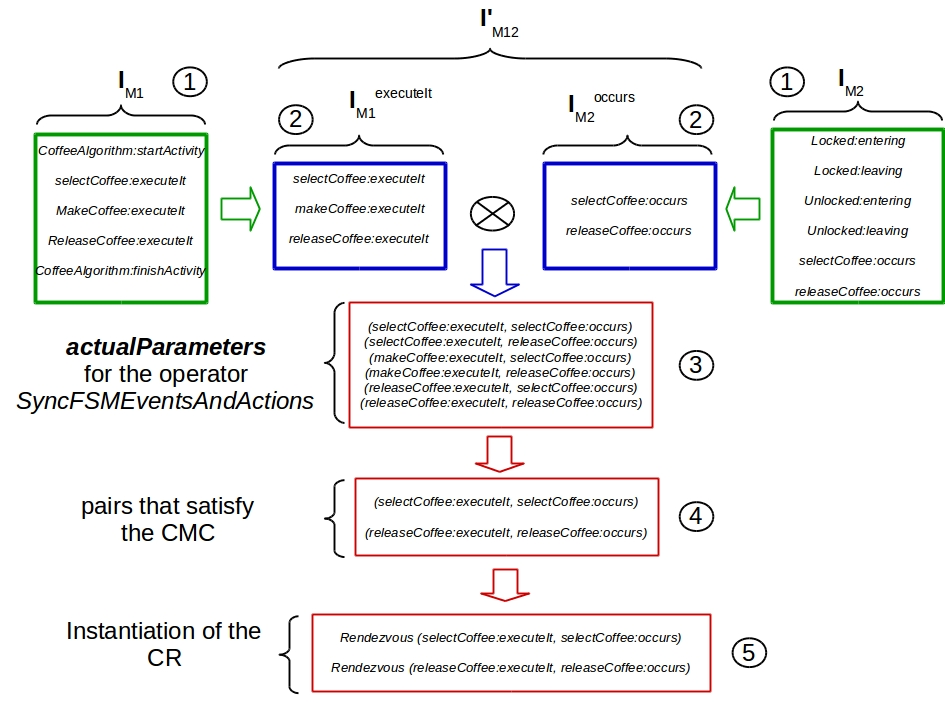
\includegraphics[width=.9\textwidth]{bcool/figs/semantics.jpg}
	\caption{Steps in the application of the \bcool specification between the models of the coffee machine}
	\label{fig:semantics}
\end{figure}



\begin{lstlisting}[language=moccml,
caption={Resulting \ccsl specification for the running example},
label={lst:runningexampleccsl}, 
basicstyle=\scriptsize\ttfamily, backgroundcolor=\color{LGrey}, numbers=left, xleftmargin=2pt]
ClockConstraintSystem SyncProductTFSM-fUMLOperatorsCoordination {
imports {
import "coffeeCoin.extendedCCSL" as coffeeCoin;
import "coffeeAlgorithm.extendedCCSL" as coffeeAlgorithm;
}
entryBlock mainBlock
Block mainBlock {
Block coffeeCoincoffeeAlgorithmsublock {
Relation SyncProductselectCoffee_startselectCoffee_occurs [ RendezVous ]
( ClockA -> "coffeeAlgorithm::selectCoffee_executeIt",
ClockB -> "coffeeCoin::selectCoffee_occurs")
Relation SyncProductreleaseCoffee_startActionreleaseCoffee_occurs [ RendezVous ]
( ClockA -> "coffeeAlgorithm::releaseCoffee_executeIt",
ClockB -> "coffeeCoin::releaseCoffee_occurs")}}
}
\end{lstlisting}    